\subsection{Tổng quan và Phân tích các phương pháp tiếp cận (Literature Review)}
\label{sec:5_1}

Dự báo lưu lượng và tình trạng ùn tắc giao thông là một bài toán chuỗi thời gian (Time-series forecasting) mang tính thách thức cao do bản chất ngẫu nhiên (stochastic) và độ phức tạp về mặt không gian của mạng lưới đường bộ. Để đánh giá tính khả thi và hiệu quả của các kiến trúc dự báo, nghiên cứu này tiến hành phân tích và so sánh các phương pháp tiếp cận hiện hành dựa trên ba tiêu chí cốt lõi: (1) Khả năng bắt giữ phụ thuộc thời gian (Temporal dependence capture), (2) Năng lực xử lý dữ liệu phi cấu trúc và đa phương thức (Unstructured/Multimodal data handling), và (3) Mục tiêu tối ưu hóa (Optimization objectives).

Việc phân tích các phương pháp từ cổ điển đến hiện đại giúp làm rõ những rào cản kỹ thuật hiện tại, từ đó củng cố cơ sở khoa học cho việc đề xuất kiến trúc Học chuyển giao lai (Hybrid Transfer RL) trong đồ án này.

\subsubsection{Tiếp cận dựa trên Thống kê truyền thống (ARIMA, SARIMA)}

\paragraph{a. Nguyên lý hoạt động và Cơ sở toán học} \mbox{} \\
Phương pháp tự hồi quy tích hợp trung bình trượt (Autoregressive Integrated Moving Average - ARIMA) và biến thể có tính mùa vụ (SARIMA) là những mô hình thống kê kinh điển nhất trong phân tích chuỗi thời gian. Nguyên lý cốt lõi của ARIMA dựa trên giả định về tính dừng (stationarity) của dữ liệu. Nghĩa là, các đặc trưng thống kê của chuỗi thời gian (như kỳ vọng, phương sai) không thay đổi theo thời gian.

Mô hình thiết lập dự báo dựa trên một tổ hợp tuyến tính bao gồm ba thành phần:
\begin{itemize}
    \item \textbf{AR (Autoregressive - Tự hồi quy):} Biểu diễn giá trị hiện tại như một hàm tuyến tính của các giá trị trong quá khứ, giúp bắt giữ quán tính của dòng xe.
    \item \textbf{I (Integrated - Tích hợp):} Sử dụng sai phân (differencing) để triệt tiêu xu hướng (trend), ép chuỗi dữ liệu giao thông phi dừng về trạng thái dừng.
    \item \textbf{MA (Moving Average - Trung bình trượt):} Khai thác mối liên hệ phụ thuộc giữa giá trị quan sát hiện tại và các sai số ngẫu nhiên (white noise) từ các dự báo trước đó.
\end{itemize}

\paragraph{b. Ưu điểm} \mbox{} \\
Đối với tiêu chí thứ nhất (bắt giữ phụ thuộc thời gian), ARIMA thực hiện rất tốt trong điều kiện dòng lưu lượng giao thông ở trạng thái dòng tự do (free-flow) hoặc biến thiên theo chu kỳ ổn định. Mô hình có tính minh bạch toán học (White-box) cao, dễ dàng diễn giải các hệ số tác động và yêu cầu chi phí tính toán cực kỳ thấp.

\paragraph{c. Hạn chế thực tiễn và Sự thất bại trước thảm họa giao thông} \mbox{} \\
Tuy nhiên, khi đối chiếu với thực tiễn mạng lưới giao thông tại TP.HCM, mô hình thống kê truyền thống bộc lộ những khuyết điểm chí mạng:
\begin{enumerate}
    \item \textbf{Sự bất lực trước "Điểm gãy" phi tuyến tính (Non-linear Structural Breaks):} ARIMA bị ràng buộc bởi giả định quan hệ tuyến tính. Trong thực tế, sự hình thành kẹt xe thảm họa (Mức 4, Mức 5) không diễn ra từ từ mà là một sự suy sụp cấu trúc đột ngột (ví dụ: một vụ tai nạn hoặc mưa lớn đổ xuống khiến vận tốc giảm từ 40 km/h xuống 5 km/h chỉ trong 2 phút). Khi đối mặt với biến động này, kết quả dự báo của ARIMA bị trễ pha (Lagging effect) nghiêm trọng. Mô hình thường dự báo kẹt xe \textit{sau khi} kẹt xe đã thực sự xảy ra, khiến giá trị cảnh báo sớm bị triệt tiêu hoàn toàn.
    \item \textbf{Khả năng xử lý dữ liệu ngoại lai kém (Tiêu chí 2):} ARIMA chỉ chấp nhận dữ liệu đầu vào là một chuỗi giá trị đơn biến (Univariate) hoặc đa biến tuyến tính. Nó hoàn toàn bất lực trong việc nhúng (embedding) các dữ liệu phi cấu trúc mang tính tâm lý và không gian như sự thay đổi thời tiết, ID phân vùng địa lý, hay mã loại đường bộ.
    \item \textbf{Sai lệch Mục tiêu Tối ưu (Tiêu chí 3):} Hàm mục tiêu của ARIMA thường là giảm thiểu sai số toàn phương trung bình (MSE). Điều này buộc mô hình phải bám sát vào nhóm dữ liệu đa số (trạng thái thông thoáng), dẫn đến việc bỏ qua các giá trị ngoại lai (Anomalies) vốn đại diện cho thảm họa giao thông.
\end{enumerate}

\begin{figure}[H]
    \centering
    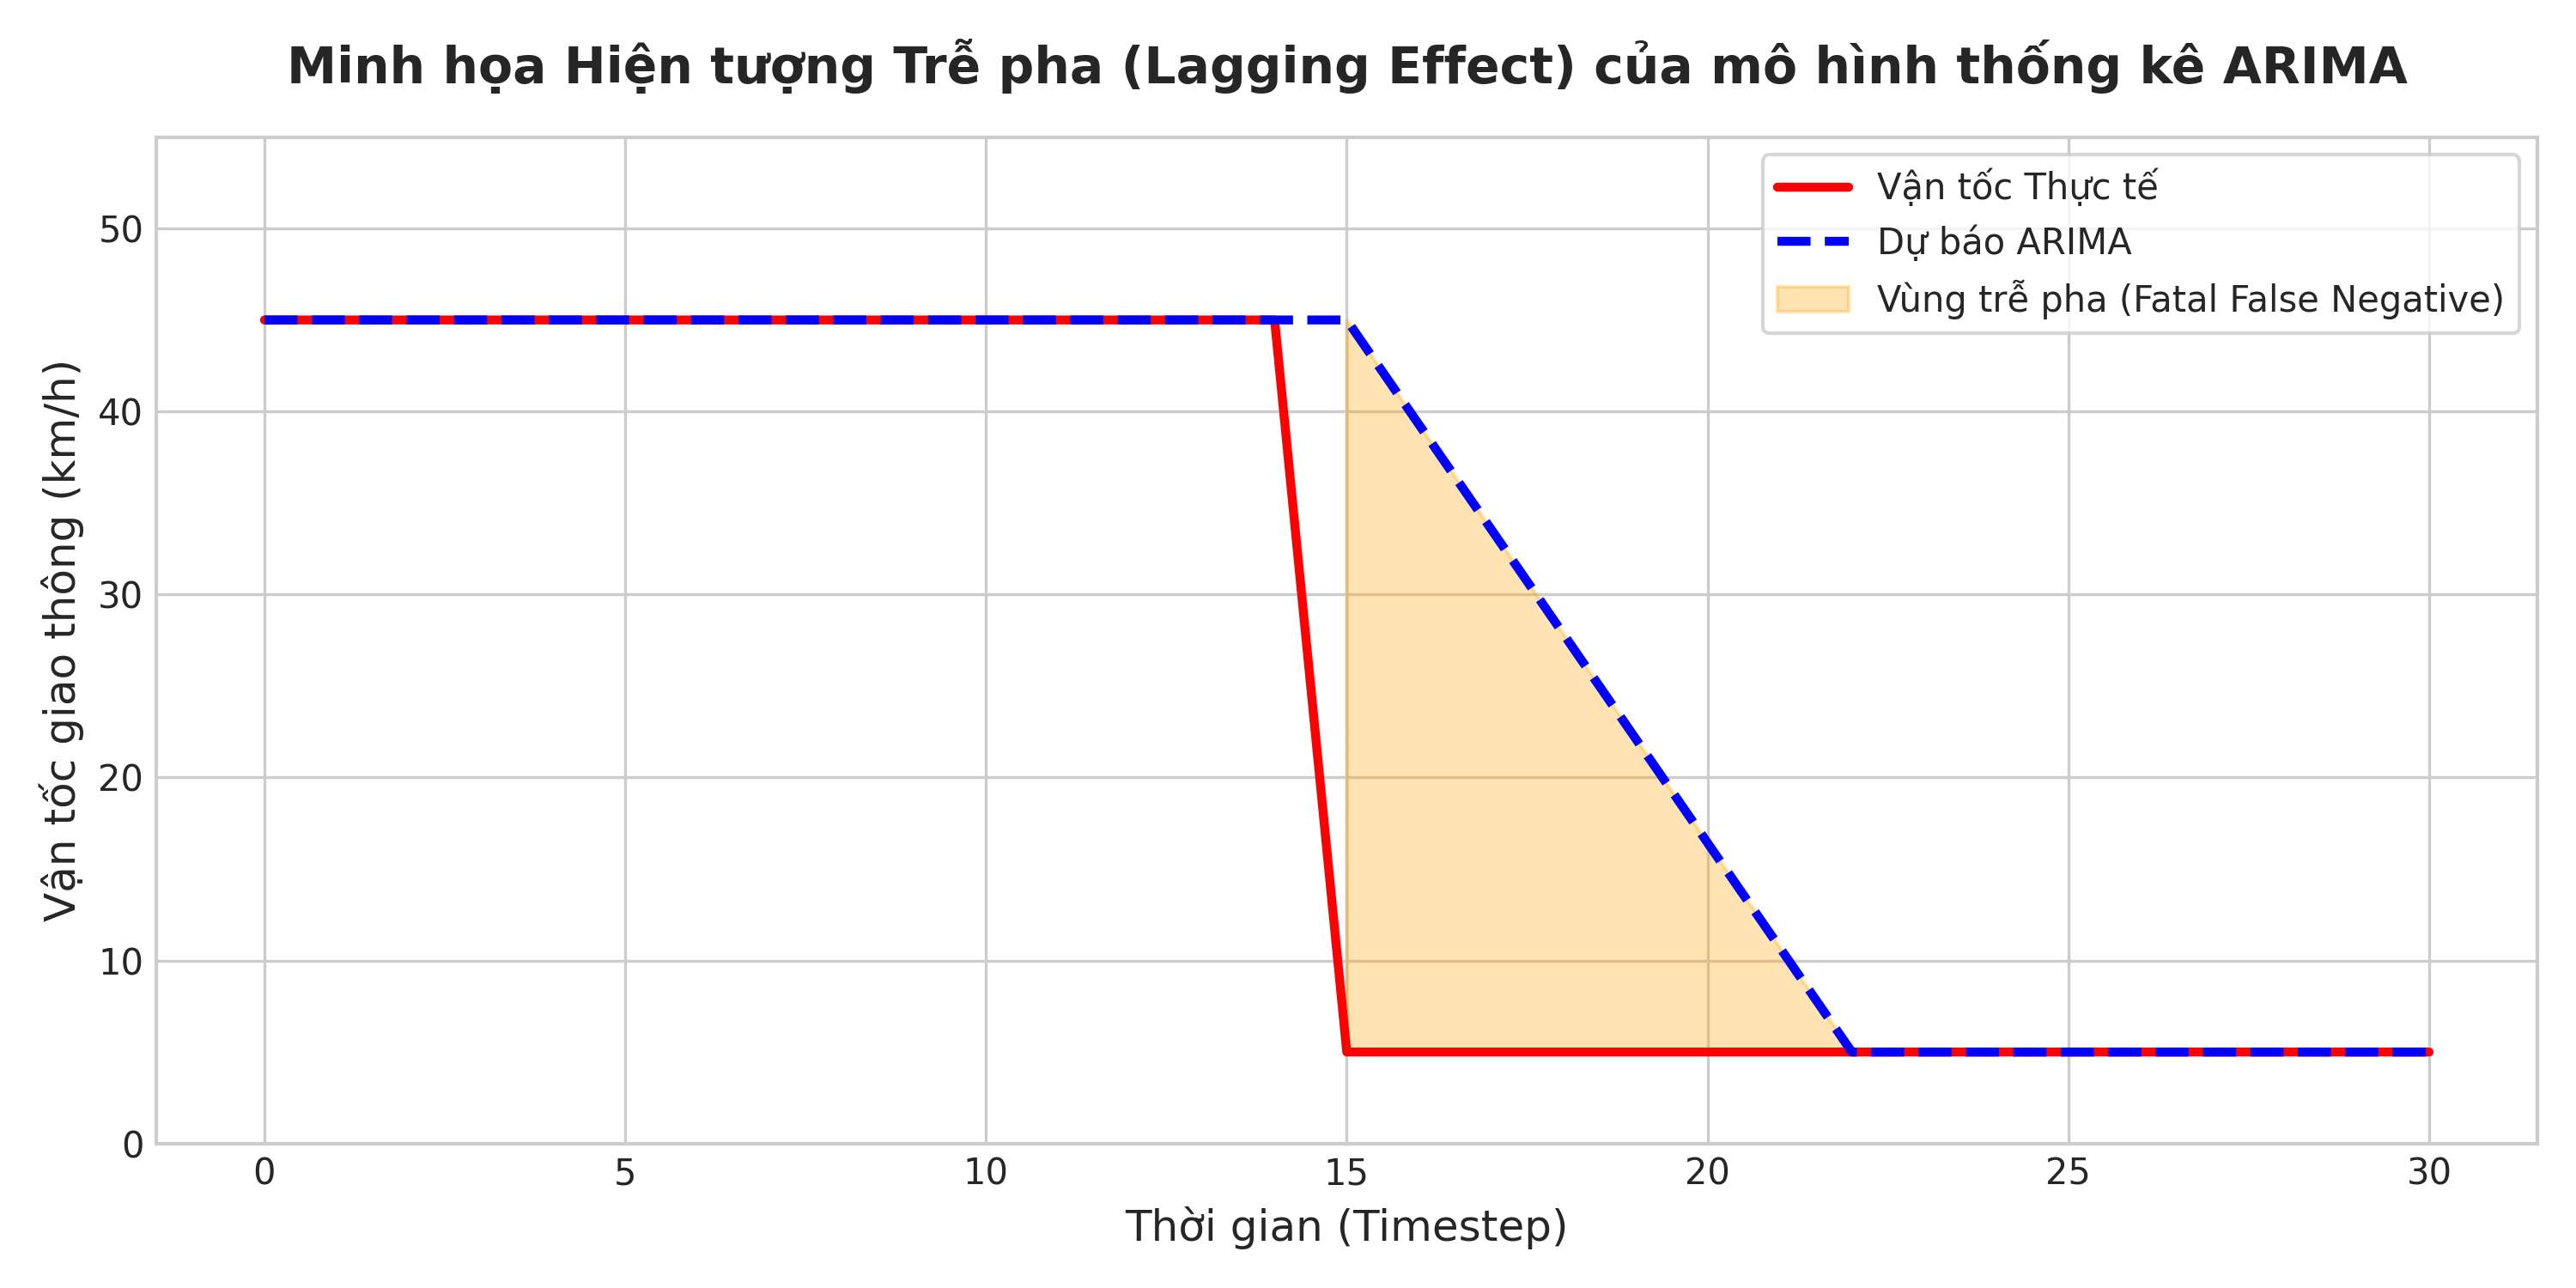
\includegraphics[width=0.8\textwidth]{Images/CH5/1.png}
    \vspace{12pt}
    \caption{Biểu đồ minh họa hiện tượng Trễ pha của mô hình ARIMA}
    \label{fig:5_1}
\end{figure}

\subsubsection{Tiếp cận dựa trên Học sâu (LSTM, CNN, T-GCN)}

Sự bùng nổ của Học sâu (Deep Learning - DL) đã mở ra một kỷ nguyên mới cho bài toán dự báo giao thông nhờ khả năng tự động trích xuất các đặc trưng phi tuyến tính phức tạp mà không cần sự can thiệp thủ công từ chuyên gia.

\begin{figure}[H]
    \centering
    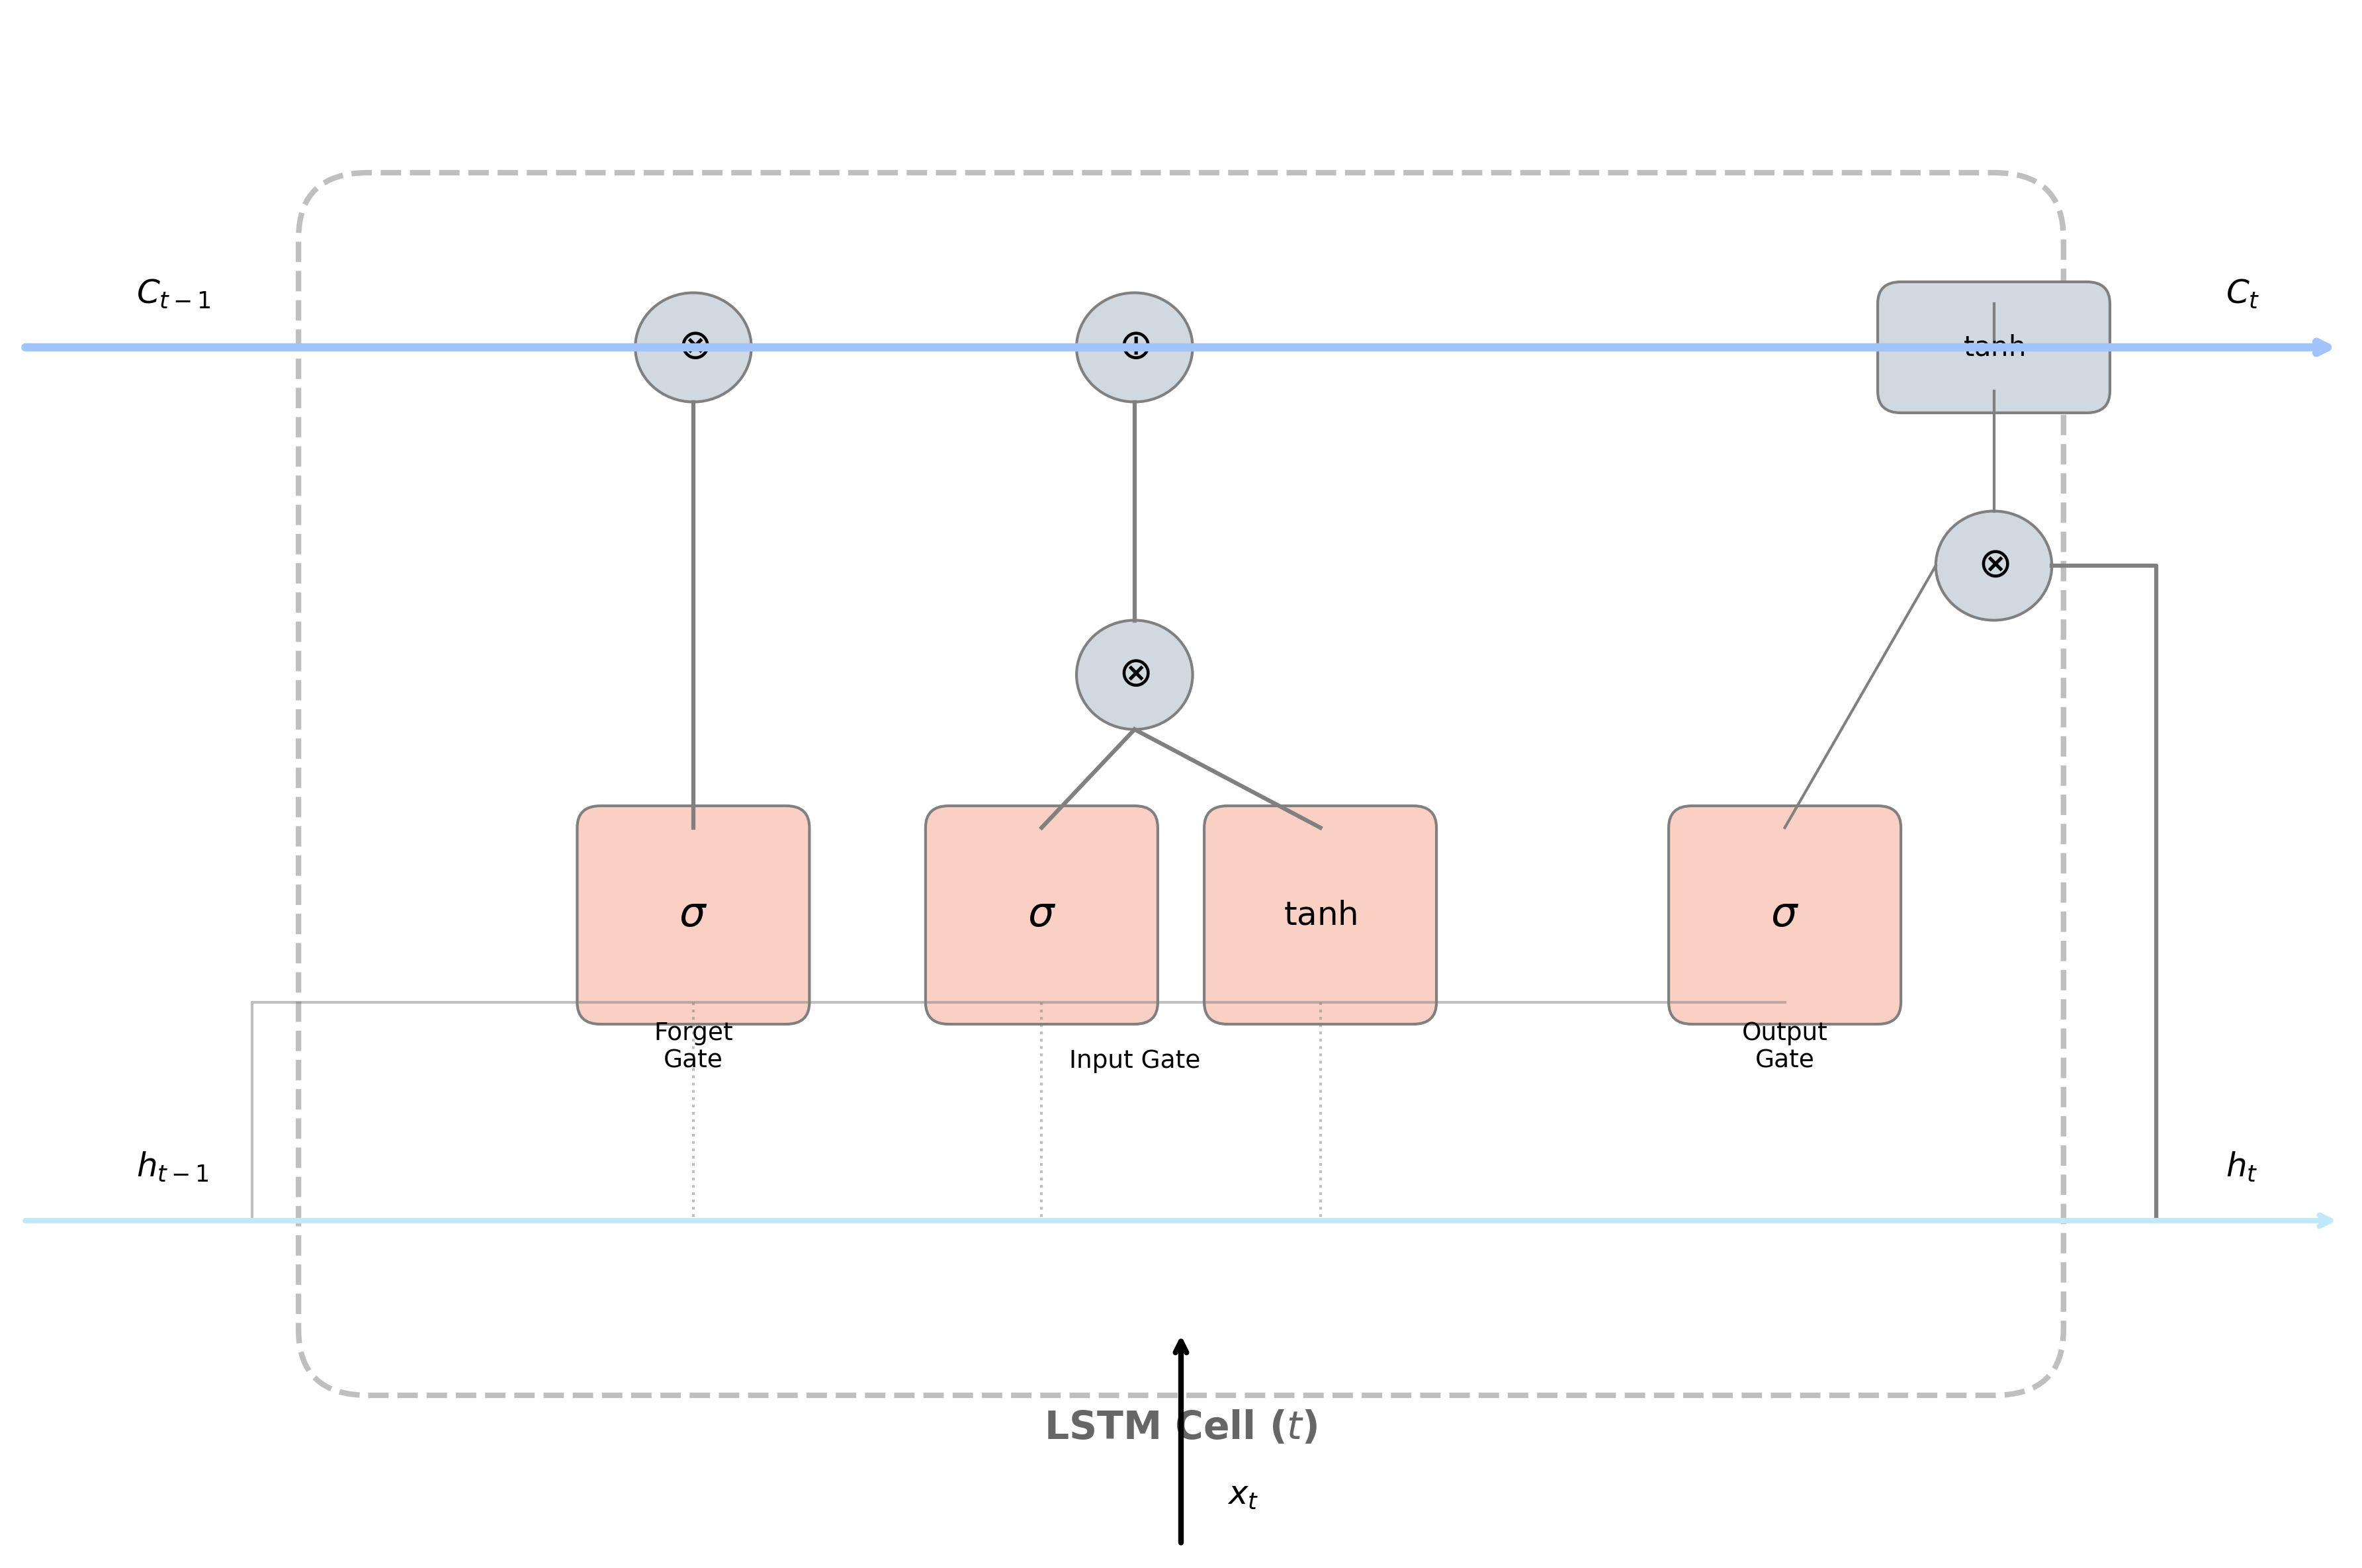
\includegraphics[width=0.8\textwidth]{Images/CH5/2.png}
    \vspace{12pt}
    \caption{Sơ đồ khối kiến trúc LSTM đơn giản}
    \label{fig:5_2}
\end{figure}

\paragraph{a. Khả năng bắt giữ phụ thuộc thời gian với mạng LSTM} \mbox{} \\
Trong các kiến trúc DL, mạng Bộ nhớ ngắn hạn dài (Long Short-Term Memory - LSTM) được xem là tiêu chuẩn vàng cho dữ liệu chuỗi thời gian. Khác với mạng nơ-ron truyền thống, LSTM giải quyết triệt để vấn đề Tiêu biến đạo hàm (Vanishing Gradient) nhờ vào cấu trúc "Tế bào nhớ" (Memory cell) và cơ chế các cổng (Gates):
\begin{itemize}
    \item \textbf{Cổng quên (Forget Gate):} Loại bỏ những thông tin không còn giá trị từ quá khứ (ví dụ: dữ liệu vận tốc của 2 tiếng trước không còn ảnh hưởng đến kẹt xe hiện tại).
    \item \textbf{Cổng nhập (Input Gate):} Cập nhật những thông tin mới quan trọng vào trạng thái tế bào.
    \item \textbf{Cổng xuất (Output Gate):} Quyết định thông tin nào sẽ được đưa ra làm đầu ra và chuyển sang bước thời gian tiếp theo.
\end{itemize}
Cơ chế này cho phép LSTM duy trì sự phụ thuộc xa (Long-term dependencies), giúp mô hình hiểu được xu hướng giao thông kéo dài qua nhiều khung giờ.

\paragraph{b. Khả năng xử lý dữ liệu phi cấu trúc và không gian (CNN, T-GCN)} \mbox{} \\
Bên cạnh yếu tố thời gian, các mô hình như Mạng nơ-ron tích chập (CNN) và Mạng tích chập đồ thị (T-GCN) được tích hợp để xử lý Phụ thuộc không gian (Spatial dependence). Trong khi CNN hiệu quả với dữ liệu dạng lưới (Grid-based), T-GCN lại tỏ ra ưu việt trong việc mô hình hóa mạng lưới đường phố dưới dạng một đồ thị (Graph), nơi các nút là các đoạn đường và cạnh là sự kết nối giao thông giữa chúng.

\paragraph{c. Phân tích khuyết điểm: Thiên kiến lớp đa số (Majority Class Bias)} \mbox{} \\
Dù mạnh mẽ hơn ARIMA, các mô hình Deep Learning chuẩn vẫn gặp phải một rào cản lớn về Mục tiêu tối ưu hóa (Tiêu chí 3) khi đối mặt với dữ liệu mất cân bằng:
\begin{enumerate}
    \item \textbf{Sự thống trị của Hàm Loss chuẩn:} Các mô hình DL thường sử dụng Mean Squared Error (MSE) hoặc Cross-Entropy làm hàm mất mát. Các hàm này tính toán giá trị trung bình trên toàn bộ tập dữ liệu. Vì trạng thái "Thông thoáng" (Lớp 0, 1, 2) chiếm đến 90-95\% dữ liệu, mô hình sẽ bị "đánh lừa" rằng việc dự báo đúng lớp đa số là cách nhanh nhất để giảm Loss xuống mức tối thiểu.
    \item \textbf{Hệ quả "Mù màu" với thảm họa:} Kết quả là mô hình đạt độ chính xác (Accuracy) tổng thể rất cao (thường > 90\%), nhưng lại có chỉ số Recall ở lớp 4 và lớp 5 cực thấp. Trong thực tế, điều này cực kỳ nguy hiểm: Hệ thống báo cáo đường thông thoáng nhưng thực tế người dùng lại bị kẹt cứng trong một vụ tắc đường vỡ trận. Đây chính là hiện tượng "Học vẹt" theo lớp đa số mà các kiến trúc DL thuần túy khó lòng vượt qua nếu không có sự can thiệp về chiến lược lấy mẫu hoặc hàm phần thưởng.
\end{enumerate}

\begin{figure}[H]
    \centering
    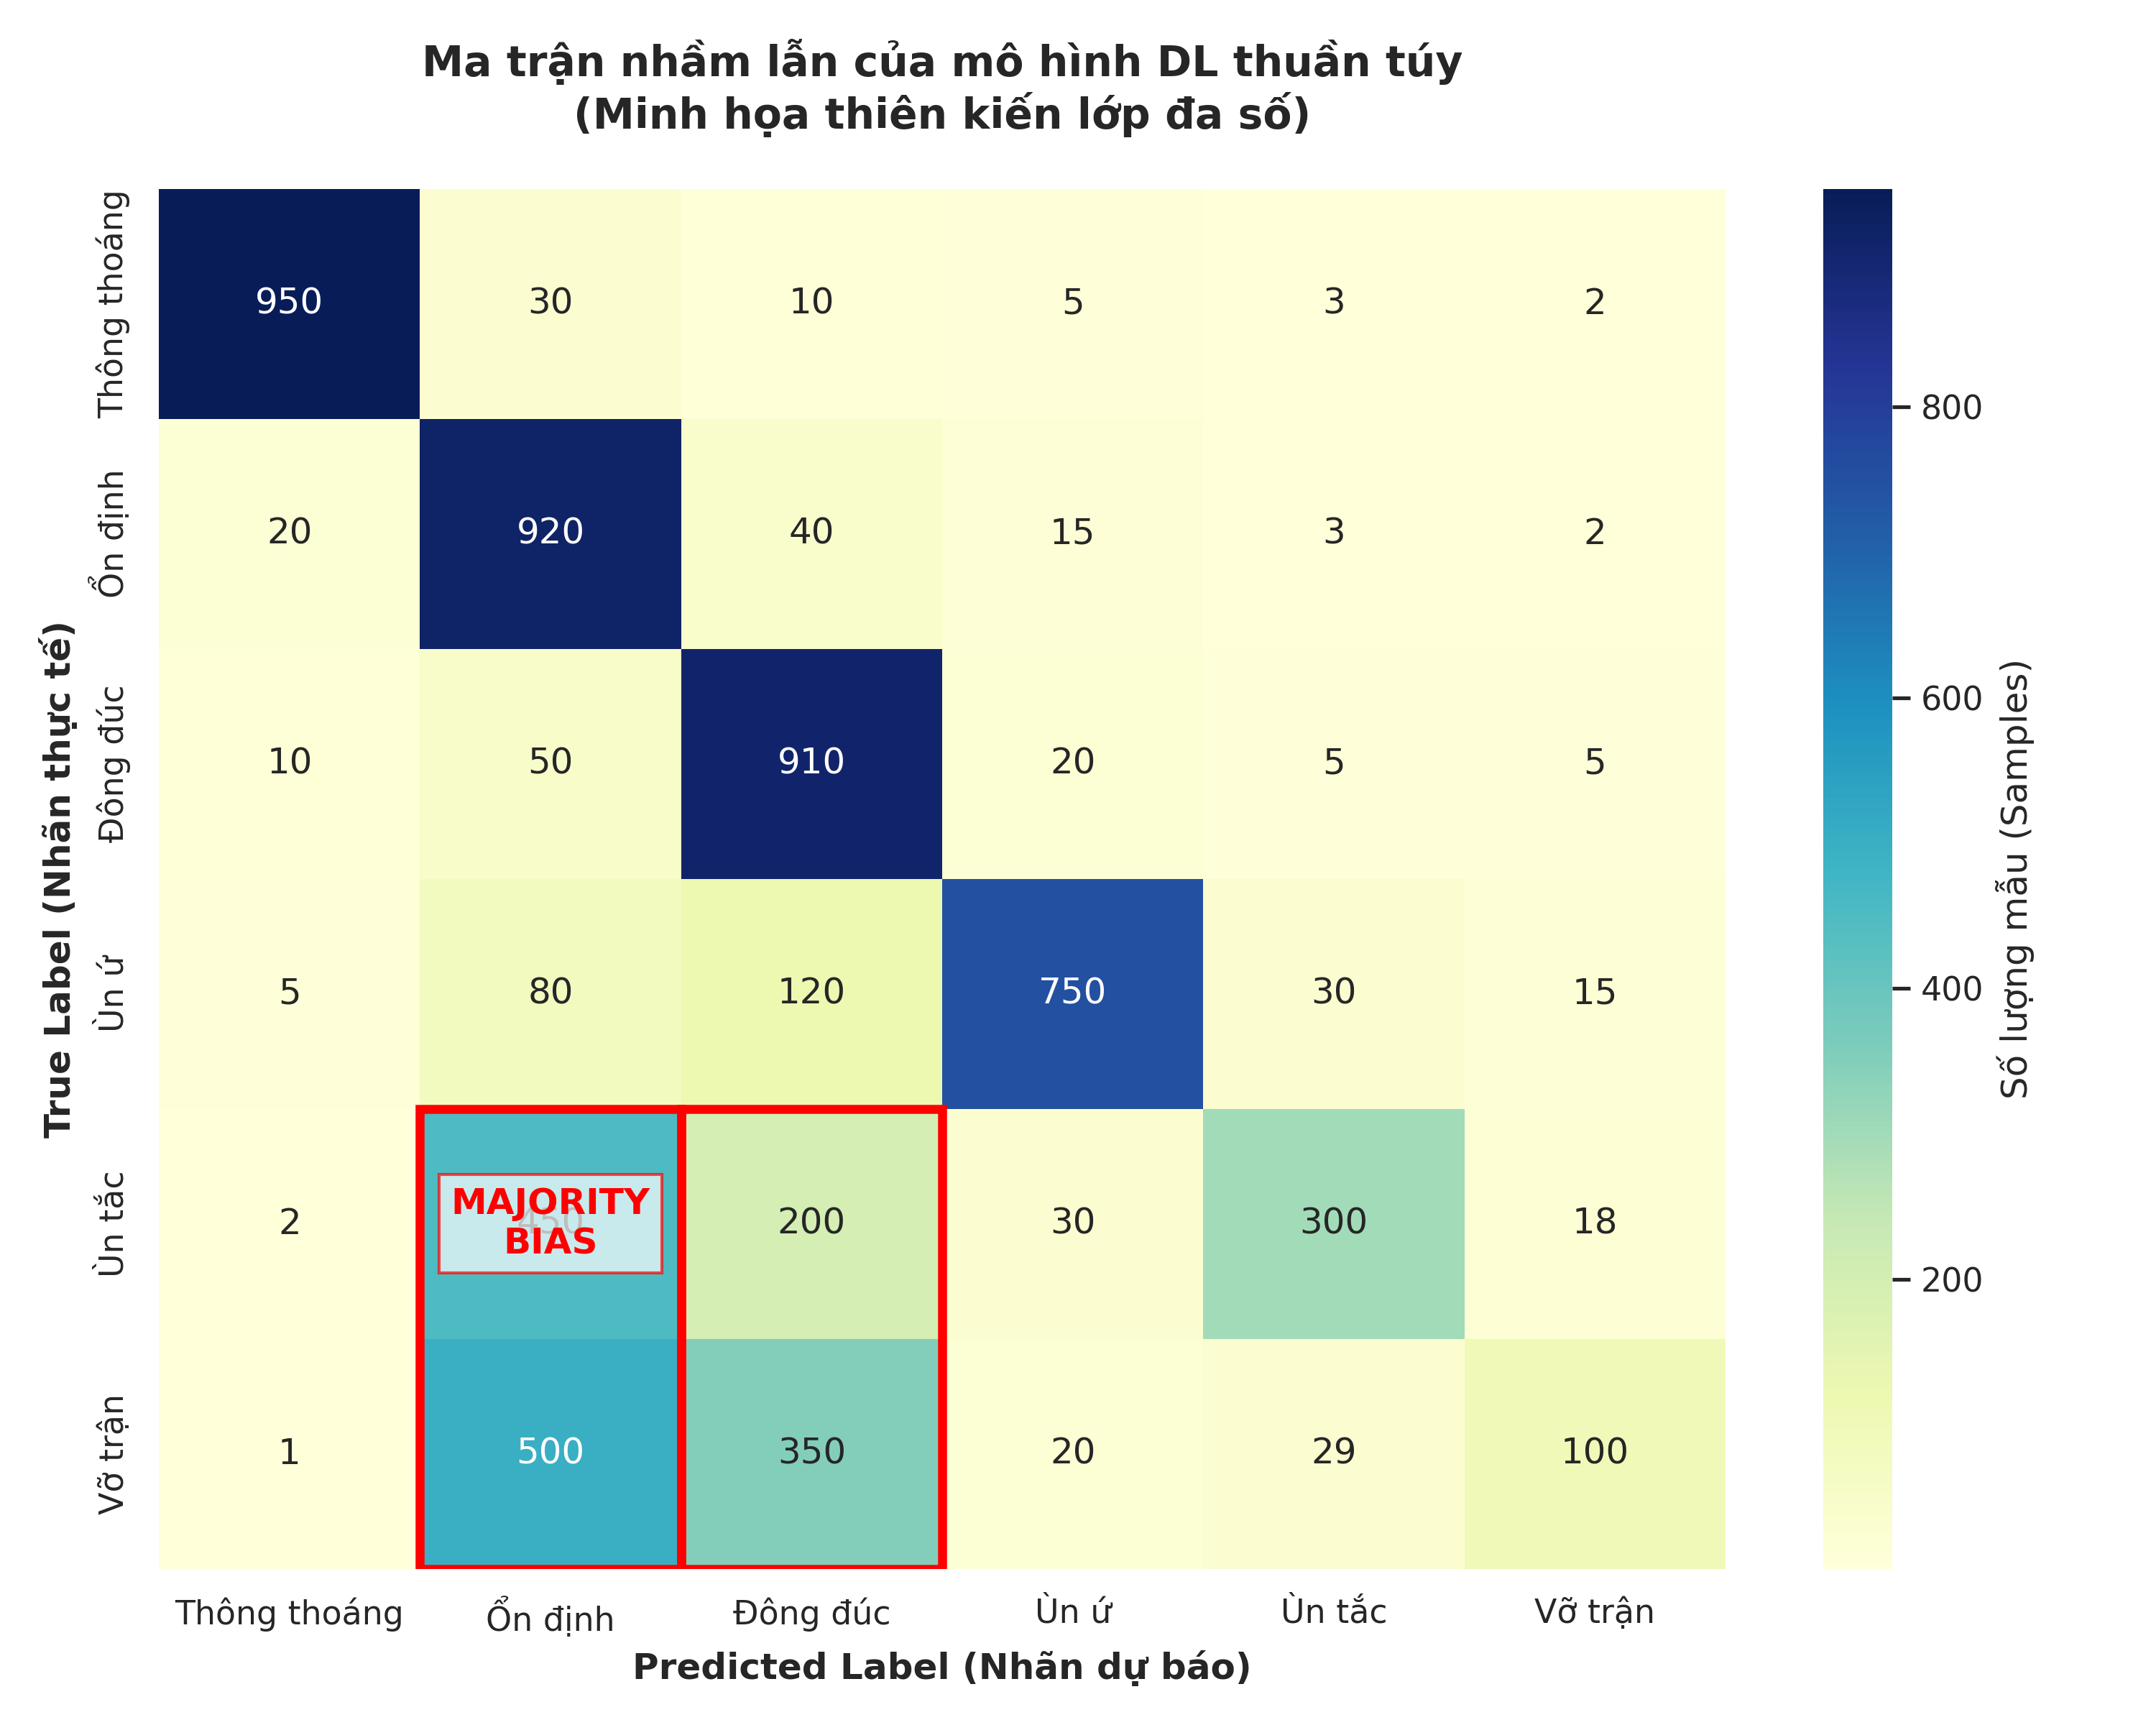
\includegraphics[width=0.8\textwidth]{Images/CH5/3.png}
    \vspace{12pt}
    \caption{Ma trận nhầm lẫn mô hình DL thuần túy}
    \label{fig:5_3}
\end{figure}

\subsubsection{Đề xuất Kiến trúc Lai (Hybrid SL-to-RL Transfer)}

Để khắc phục triệt để sự "trễ pha" của mô hình thống kê (ARIMA) và "thiên kiến lớp đa số" của mô hình Deep Learning chuẩn (LSTM), đồ án đề xuất một kiến trúc lai đột phá: \textbf{Hybrid SL-to-RL Transfer}. Phương pháp này tái định nghĩa bài toán dự báo giao thông không chỉ là việc khớp đường cong dữ liệu (curve-fitting), mà là một quá trình ra quyết định tối ưu tuần tự (Sequential Decision Making).

Kiến trúc đề xuất là sự giao thoa giữa khả năng trích xuất đặc trưng của \textbf{Học có giám sát (Supervised Learning - SL)} và cơ chế định hướng mục tiêu của \textbf{Học tăng cường sâu (Deep Reinforcement Learning - DRL)}, bao gồm các thành phần cốt lõi sau:

\paragraph{a. Cấu trúc mạng Trích xuất Đặc trưng Đa nhánh (Multi-branch Fusion Network)} \mbox{} \\
Hệ thống sử dụng một mạng Nơ-ron tùy chỉnh (đóng vai trò là mô hình SL cơ sở và mạng Q-Network sau này) bao gồm ba nhánh song song, chịu trách nhiệm xử lý các luồng dữ liệu dị đồng nhất:
\begin{enumerate}
    \item \textbf{Nhánh Đặc trưng Động (Dynamic Branch):} Xử lý luồng dữ liệu chuỗi thời gian (vận tốc, gia tốc, tỷ lệ trễ) thông qua cấu trúc LSTM 2 lớp (với $hidden\_dim=64$). Cấu trúc này giúp trích xuất quán tính giao thông và bắt sóng xung kích khi vận tốc thay đổi.
    \item \textbf{Nhánh Ngữ cảnh Phân loại (Categorical Branch):} Thay vì sử dụng One-hot encoding gây hiện tượng bùng nổ số chiều và ma trận thưa, đồ án áp dụng Tầng Nhúng không gian (Embedding Layers với $dim=8$). Kỹ thuật này ánh xạ các định danh rời rạc (ID đoạn đường, mã Phường/Xã) thành các vector dày đặc liên tục, giúp mạng nơ-ron học được tính tương đồng về không gian giữa các khu vực địa lý lân cận.
    \item \textbf{Nhánh Đặc trưng Tĩnh (Static Branch):} Sử dụng mạng nơ-ron truyền thẳng (Feed-Forward Neural Network - FNN) để xử lý các thuộc tính vật lý bất biến (tọa độ GPS, số làn xe, chiều dài đoạn đường).
\end{enumerate}
Đầu ra của ba nhánh này được kết hợp (concatenate) tạo thành một vector đại diện toàn cục (Fusion Vector) trước khi đi qua các tầng phân loại cuối cùng (Classifier).

\begin{figure}[H]
    \centering
    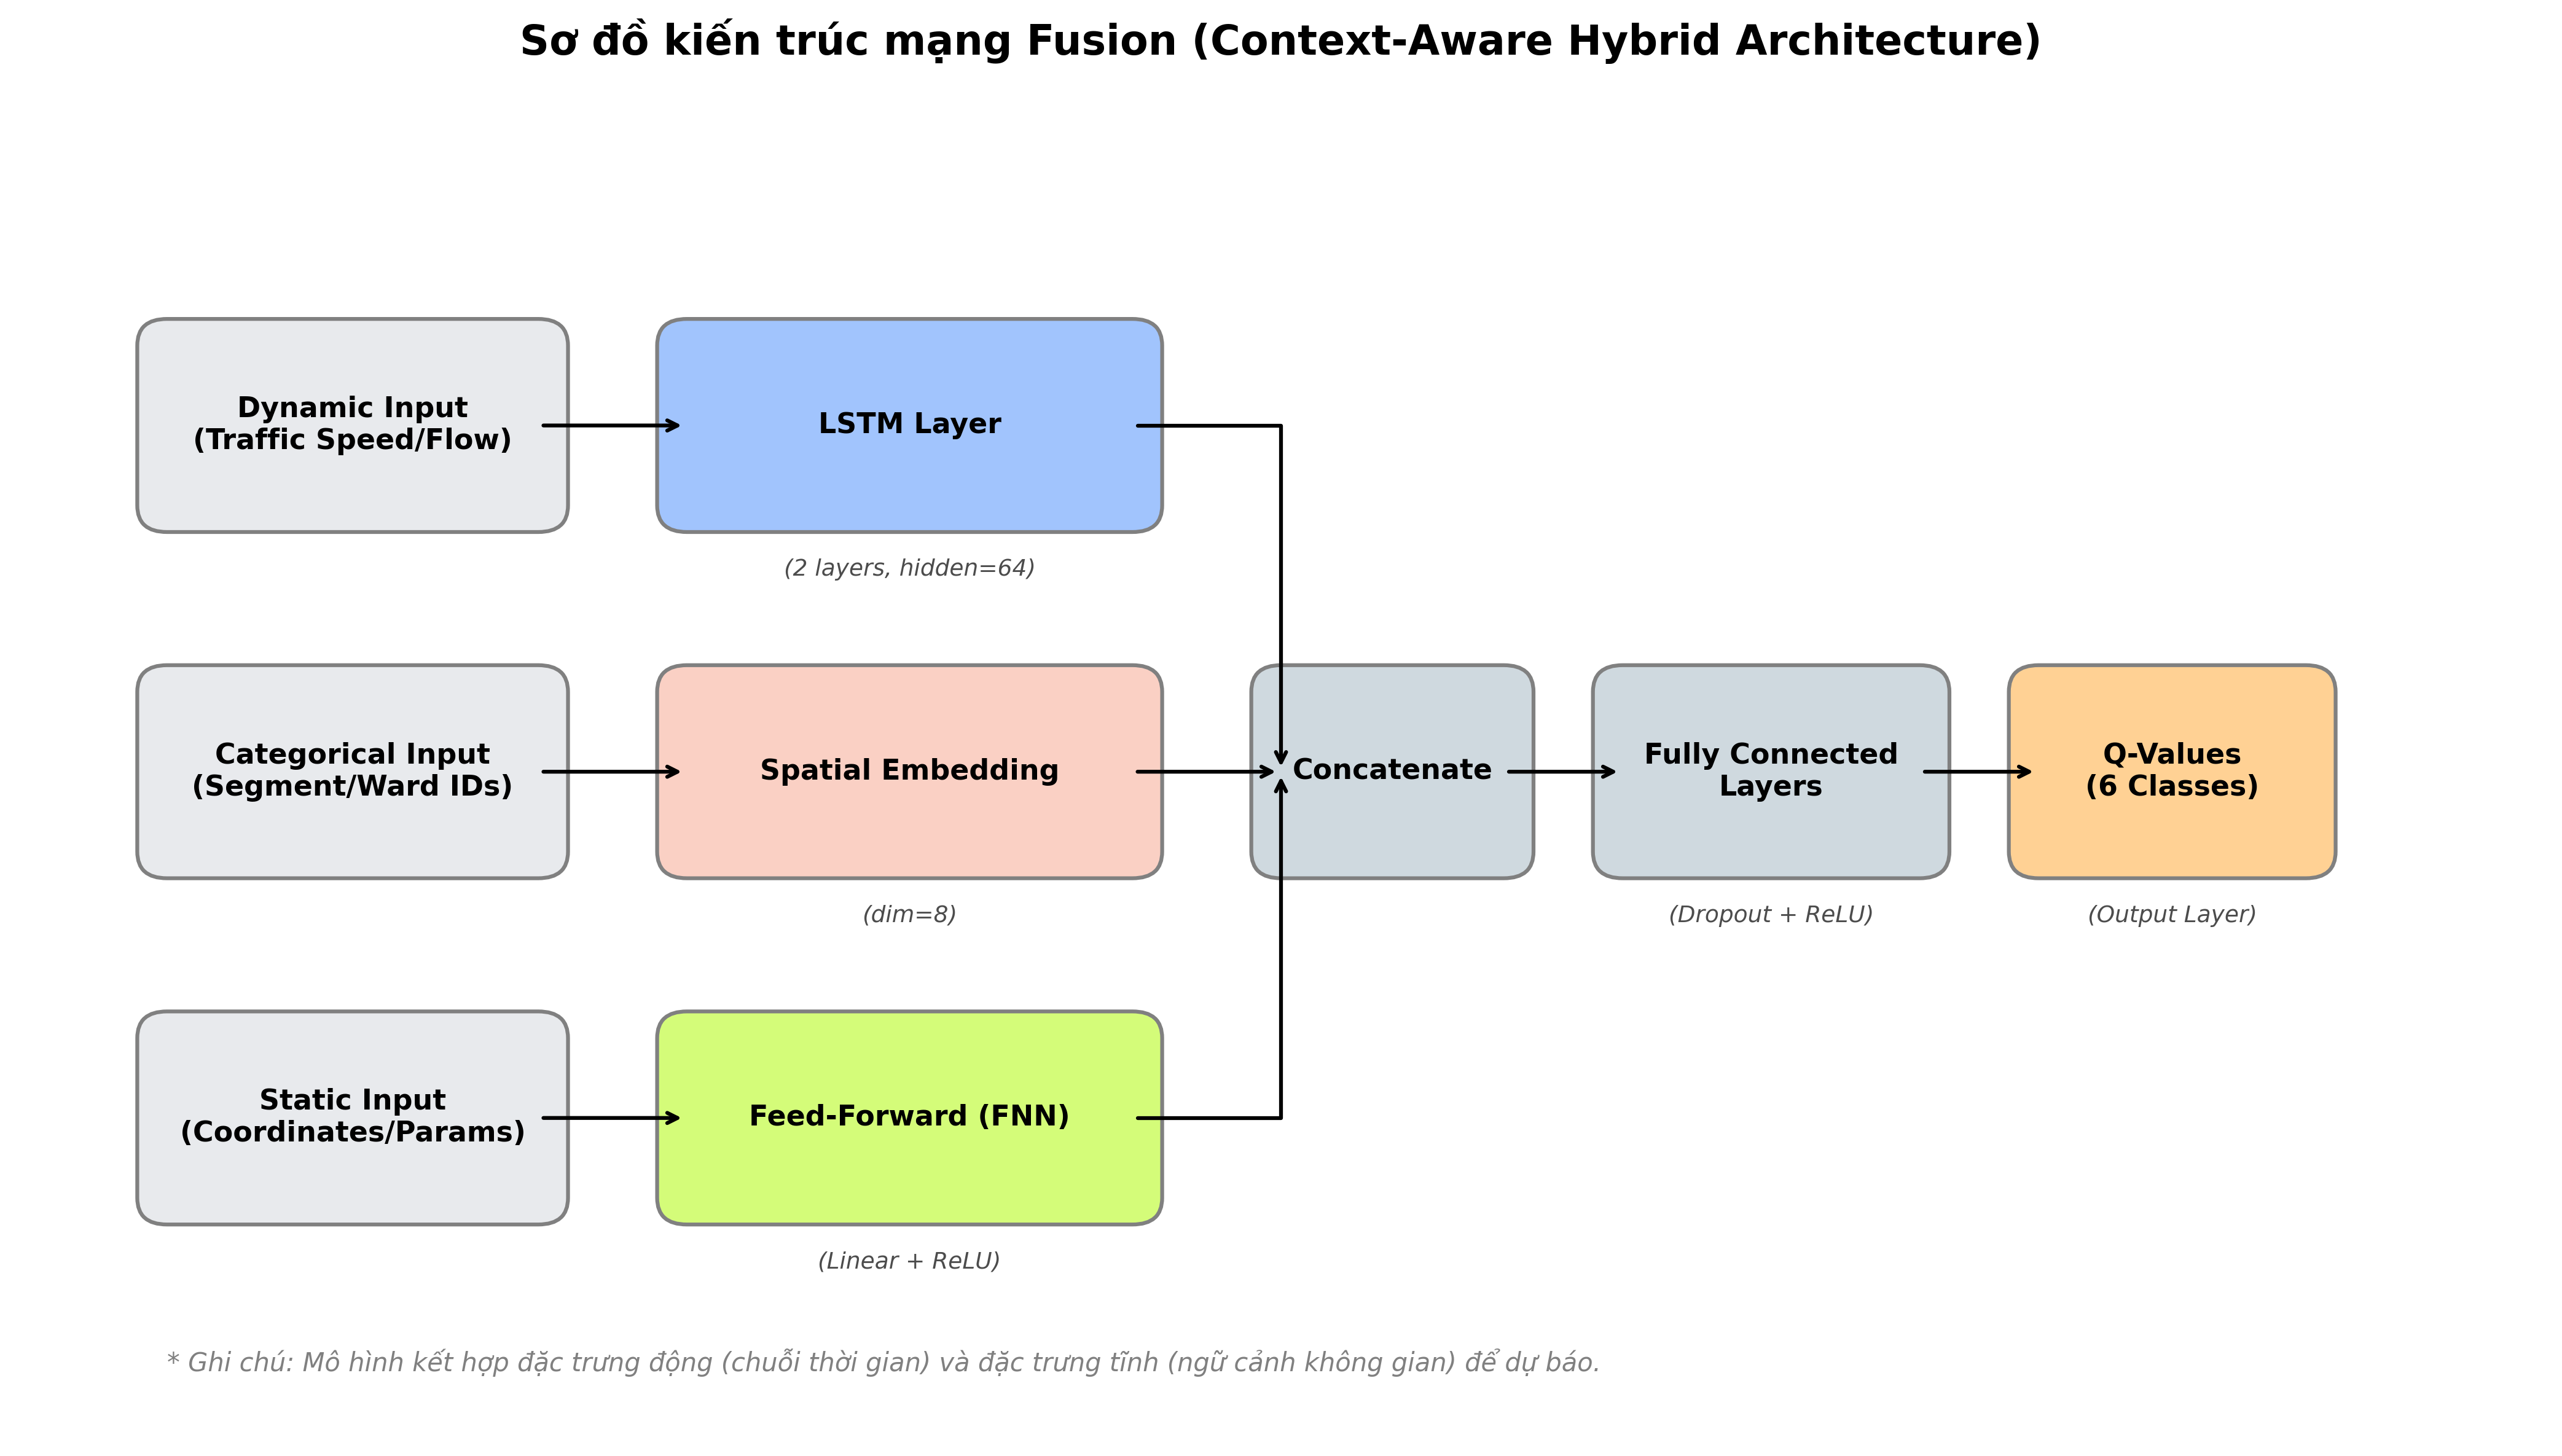
\includegraphics[width=0.8\textwidth]{Images/CH5/4.png}
    \vspace{6pt}
    \caption{Sơ đồ kiển trúc tổng thể}
    \label{fig:5_4}
\end{figure}

\paragraph{b. Cơ chế Học chuyển giao và Khởi động ấm (SL-to-RL Warmstart)} \mbox{} \\
Một nhược điểm chí mạng của Học tăng cường (RL) là vấn đề "Khởi động lạnh" (Cold Start). Nếu khởi tạo trọng số ngẫu nhiên, Agent sẽ mất lượng lớn thời gian để mò mẫm các quy luật vật lý cơ bản, dễ dẫn đến mất hội tụ. Để giải quyết, đồ án áp dụng chiến lược Warmstart: Mạng Fusion đa nhánh ban đầu được tiền huấn luyện (Pre-train) hoàn toàn bằng phương pháp Học có giám sát (SL) với hàm mất mát Cross-Entropy. Sau khi mạng đã có "bản năng" nhận diện giao thông cơ bản, toàn bộ trọng số (weights) này được chuyển giao (Transfer) và nạp trực tiếp vào Đặc vụ DQN trước khi bắt đầu quá trình tinh chỉnh (Fine-tuning) bằng RL. Điều này giúp Agent có một xuất phát điểm cực kỳ vững chắc.

\paragraph{c. Tối ưu hóa với Double DQN và Hàm Phần thưởng Không đối xứng (Asymmetric Reward Shaping)} \mbox{} \\
Đặc vụ (Agent) sử dụng thuật toán Double DQN kết hợp bộ nhớ kinh nghiệm (Replay Buffer) dung lượng $100.000$ mẫu. Việc sử dụng mạng mục tiêu (Target Network) tách biệt với mạng chính sách (Policy Network) giúp triệt tiêu hội chứng ảo tưởng sức mạnh (Overestimation Bias) vốn thường gặp ở Q-Learning truyền thống.

Tuy nhiên, "trái tim" và bí quyết thành công của hệ thống nằm ở thiết kế Hàm phần thưởng (Reward Shaping). Nhằm triệt tiêu thiên kiến lớp đa số (mô hình thích đoán kẹt xe thành thông thoáng để an toàn), đồ án thiết kế một cơ chế điểm phạt phi tuyến tính và không đối xứng:
\begin{itemize}
    \item \textbf{Thưởng khích lệ:} Nếu dự báo chính xác mức độ kẹt xe, Agent nhận $+2$ điểm.
    \item \textbf{Phạt cảnh cáo:} Nếu dự báo sai lệch nhẹ (chênh lệch 1 mức, ví dụ thực tế Mức 2 nhưng đoán Mức 1), Agent bị trừ $-1$ điểm. Đây là mức sai số có thể chấp nhận được trong thực tế.
    \item \textbf{Phạt sinh tử (Fatal Penalty):} Nếu hệ thống đối mặt với thảm họa (Thực tế là Mức 4 hoặc 5) nhưng Agent báo cáo sai thành thông thoáng (Mức 0 hoặc 1), mức phạt sẽ tăng vọt lên từ $-10$ đến $-20$ điểm.
\end{itemize}
Cơ chế "đòn bẩy" này tạo ra một rào cản tâm lý, ép Agent phải nhạy bén tối đa với các tín hiệu thảm họa, chấp nhận hy sinh một phần nhỏ độ chính xác ở các lớp thông thoáng để bảo vệ năng lực cảnh báo sớm cho người dùng.

\begin{figure}[H]
    \centering
    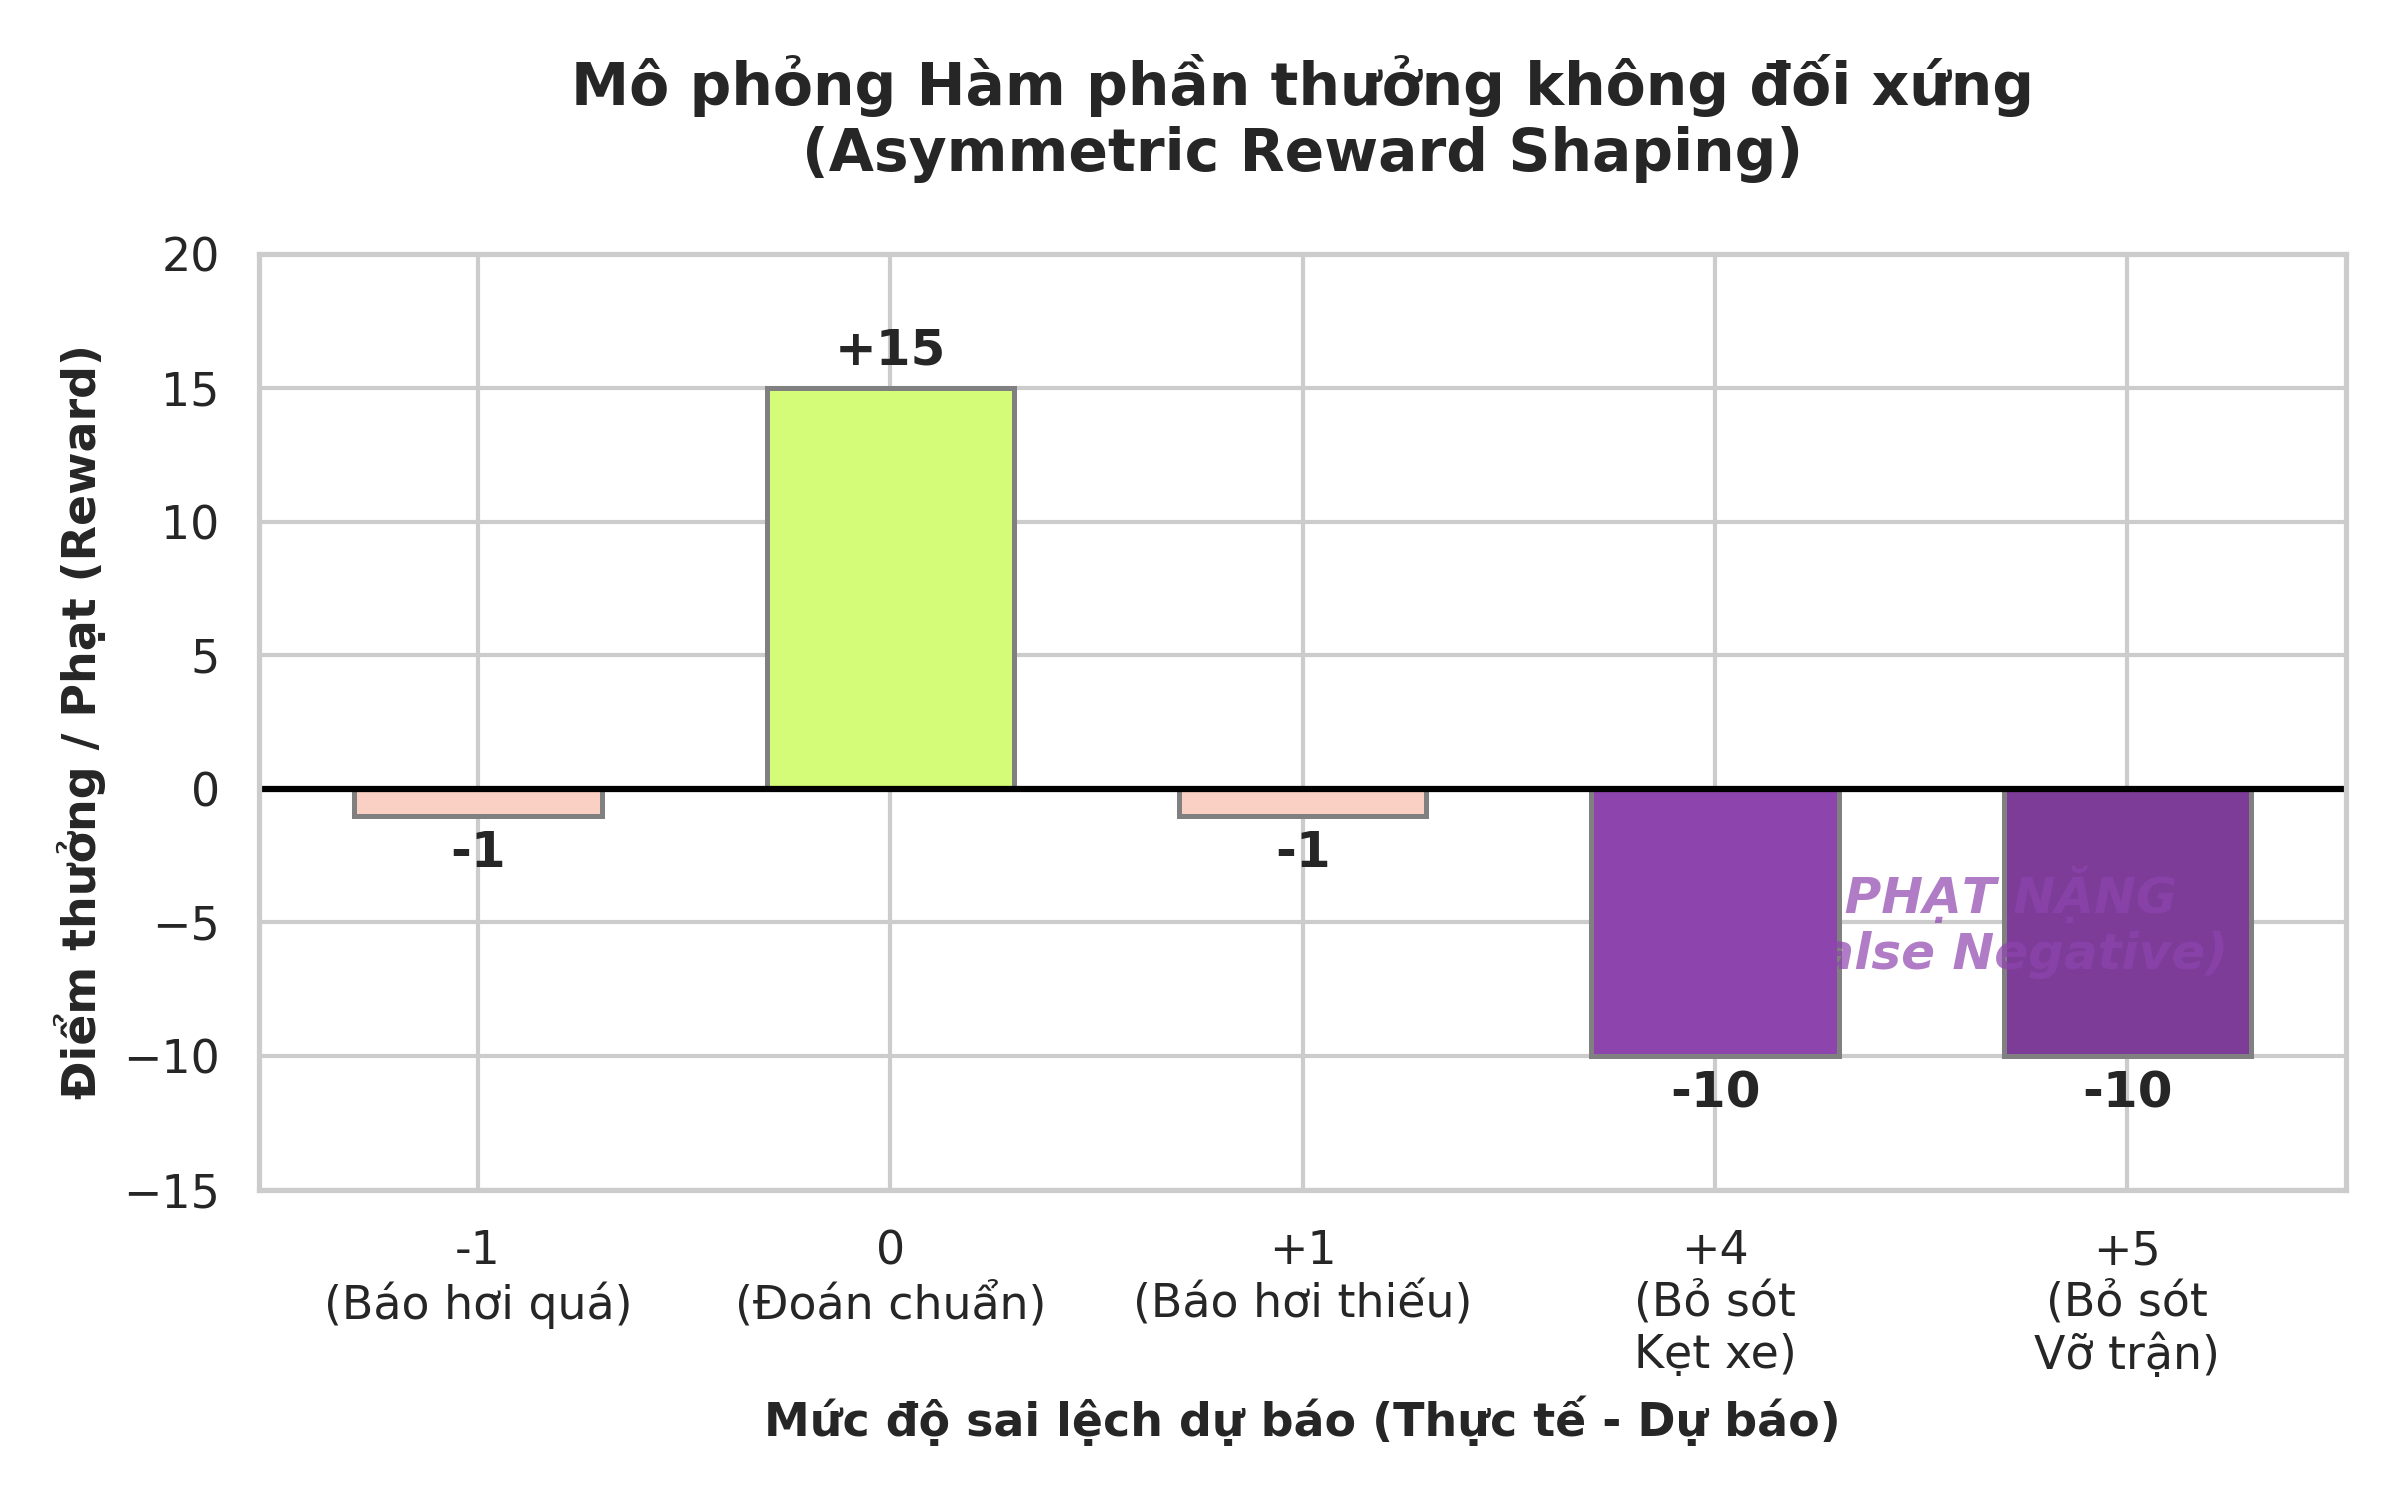
\includegraphics[width=0.8\textwidth]{Images/CH5/5.png}
    \vspace{6pt}
    \caption{Đồ thị hàm phần thưởng}
    \label{fig:5_5}
\end{figure}

\paragraph{d. Đánh giá ưu điểm và thách thức} \mbox{} \\
\begin{itemize}
    \item \textbf{Ưu điểm vượt trội:} Kiến trúc lai đạt được cả hai mục tiêu cực hạn: Tốc độ hội tụ nhanh (nhờ tri thức tiền huấn luyện từ Warmstart) và năng lực thu hồi (Recall) xuất sắc tại các lớp kẹt xe nặng (nhờ Hàm thưởng không đối xứng ép buộc Agent chú ý vào các trường hợp ngoại lai).
    \item \textbf{Thách thức:} Quá trình tinh chỉnh các siêu tham số của hàm thưởng (tỷ lệ phạt giữa -10 và -20) đòi hỏi phải thử nghiệm (trial-and-error) liên tục để tránh việc Agent rơi vào thái cực ngược lại là chứng "hoang tưởng" (luôn dự báo kẹt xe). Ngoài ra, cấu trúc Double DQN tiêu tốn bộ nhớ và thời gian tính toán cao hơn so với mô hình giám sát thuần túy.
\end{itemize}
